% Options for packages loaded elsewhere
\PassOptionsToPackage{unicode}{hyperref}
\PassOptionsToPackage{hyphens}{url}
%
\documentclass[
  ignorenonframetext,
]{beamer}
\usepackage{pgfpages}
\setbeamertemplate{caption}[numbered]
\setbeamertemplate{caption label separator}{: }
\setbeamercolor{caption name}{fg=normal text.fg}
\beamertemplatenavigationsymbolsempty
% Prevent slide breaks in the middle of a paragraph
\widowpenalties 1 10000
\raggedbottom
\setbeamertemplate{part page}{
  \centering
  \begin{beamercolorbox}[sep=16pt,center]{part title}
    \usebeamerfont{part title}\insertpart\par
  \end{beamercolorbox}
}
\setbeamertemplate{section page}{
  \centering
  \begin{beamercolorbox}[sep=12pt,center]{part title}
    \usebeamerfont{section title}\insertsection\par
  \end{beamercolorbox}
}
\setbeamertemplate{subsection page}{
  \centering
  \begin{beamercolorbox}[sep=8pt,center]{part title}
    \usebeamerfont{subsection title}\insertsubsection\par
  \end{beamercolorbox}
}
\AtBeginPart{
  \frame{\partpage}
}
\AtBeginSection{
  \ifbibliography
  \else
    \frame{\sectionpage}
  \fi
}
\AtBeginSubsection{
  \frame{\subsectionpage}
}
\usepackage{lmodern}
\usepackage{amssymb,amsmath}
\usepackage{ifxetex,ifluatex}
\ifnum 0\ifxetex 1\fi\ifluatex 1\fi=0 % if pdftex
  \usepackage[T1]{fontenc}
  \usepackage[utf8]{inputenc}
  \usepackage{textcomp} % provide euro and other symbols
\else % if luatex or xetex
  \usepackage{unicode-math}
  \defaultfontfeatures{Scale=MatchLowercase}
  \defaultfontfeatures[\rmfamily]{Ligatures=TeX,Scale=1}
\fi
\usetheme[]{metropolis}
% Use upquote if available, for straight quotes in verbatim environments
\IfFileExists{upquote.sty}{\usepackage{upquote}}{}
\IfFileExists{microtype.sty}{% use microtype if available
  \usepackage[]{microtype}
  \UseMicrotypeSet[protrusion]{basicmath} % disable protrusion for tt fonts
}{}
\makeatletter
\@ifundefined{KOMAClassName}{% if non-KOMA class
  \IfFileExists{parskip.sty}{%
    \usepackage{parskip}
  }{% else
    \setlength{\parindent}{0pt}
    \setlength{\parskip}{6pt plus 2pt minus 1pt}}
}{% if KOMA class
  \KOMAoptions{parskip=half}}
\makeatother
\usepackage{xcolor}
\IfFileExists{xurl.sty}{\usepackage{xurl}}{} % add URL line breaks if available
\IfFileExists{bookmark.sty}{\usepackage{bookmark}}{\usepackage{hyperref}}
\hypersetup{
  pdftitle={Análise de imagem no Rstudio},
  pdfauthor={Ana, João, Laura, Leonardo e Paulo},
  hidelinks,
  pdfcreator={LaTeX via pandoc}}
\urlstyle{same} % disable monospaced font for URLs
\newif\ifbibliography
\usepackage{color}
\usepackage{fancyvrb}
\newcommand{\VerbBar}{|}
\newcommand{\VERB}{\Verb[commandchars=\\\{\}]}
\DefineVerbatimEnvironment{Highlighting}{Verbatim}{commandchars=\\\{\}}
% Add ',fontsize=\small' for more characters per line
\usepackage{framed}
\definecolor{shadecolor}{RGB}{248,248,248}
\newenvironment{Shaded}{\begin{snugshade}}{\end{snugshade}}
\newcommand{\AlertTok}[1]{\textcolor[rgb]{0.94,0.16,0.16}{#1}}
\newcommand{\AnnotationTok}[1]{\textcolor[rgb]{0.56,0.35,0.01}{\textbf{\textit{#1}}}}
\newcommand{\AttributeTok}[1]{\textcolor[rgb]{0.77,0.63,0.00}{#1}}
\newcommand{\BaseNTok}[1]{\textcolor[rgb]{0.00,0.00,0.81}{#1}}
\newcommand{\BuiltInTok}[1]{#1}
\newcommand{\CharTok}[1]{\textcolor[rgb]{0.31,0.60,0.02}{#1}}
\newcommand{\CommentTok}[1]{\textcolor[rgb]{0.56,0.35,0.01}{\textit{#1}}}
\newcommand{\CommentVarTok}[1]{\textcolor[rgb]{0.56,0.35,0.01}{\textbf{\textit{#1}}}}
\newcommand{\ConstantTok}[1]{\textcolor[rgb]{0.00,0.00,0.00}{#1}}
\newcommand{\ControlFlowTok}[1]{\textcolor[rgb]{0.13,0.29,0.53}{\textbf{#1}}}
\newcommand{\DataTypeTok}[1]{\textcolor[rgb]{0.13,0.29,0.53}{#1}}
\newcommand{\DecValTok}[1]{\textcolor[rgb]{0.00,0.00,0.81}{#1}}
\newcommand{\DocumentationTok}[1]{\textcolor[rgb]{0.56,0.35,0.01}{\textbf{\textit{#1}}}}
\newcommand{\ErrorTok}[1]{\textcolor[rgb]{0.64,0.00,0.00}{\textbf{#1}}}
\newcommand{\ExtensionTok}[1]{#1}
\newcommand{\FloatTok}[1]{\textcolor[rgb]{0.00,0.00,0.81}{#1}}
\newcommand{\FunctionTok}[1]{\textcolor[rgb]{0.00,0.00,0.00}{#1}}
\newcommand{\ImportTok}[1]{#1}
\newcommand{\InformationTok}[1]{\textcolor[rgb]{0.56,0.35,0.01}{\textbf{\textit{#1}}}}
\newcommand{\KeywordTok}[1]{\textcolor[rgb]{0.13,0.29,0.53}{\textbf{#1}}}
\newcommand{\NormalTok}[1]{#1}
\newcommand{\OperatorTok}[1]{\textcolor[rgb]{0.81,0.36,0.00}{\textbf{#1}}}
\newcommand{\OtherTok}[1]{\textcolor[rgb]{0.56,0.35,0.01}{#1}}
\newcommand{\PreprocessorTok}[1]{\textcolor[rgb]{0.56,0.35,0.01}{\textit{#1}}}
\newcommand{\RegionMarkerTok}[1]{#1}
\newcommand{\SpecialCharTok}[1]{\textcolor[rgb]{0.00,0.00,0.00}{#1}}
\newcommand{\SpecialStringTok}[1]{\textcolor[rgb]{0.31,0.60,0.02}{#1}}
\newcommand{\StringTok}[1]{\textcolor[rgb]{0.31,0.60,0.02}{#1}}
\newcommand{\VariableTok}[1]{\textcolor[rgb]{0.00,0.00,0.00}{#1}}
\newcommand{\VerbatimStringTok}[1]{\textcolor[rgb]{0.31,0.60,0.02}{#1}}
\newcommand{\WarningTok}[1]{\textcolor[rgb]{0.56,0.35,0.01}{\textbf{\textit{#1}}}}
\usepackage{graphicx,grffile}
\makeatletter
\def\maxwidth{\ifdim\Gin@nat@width>\linewidth\linewidth\else\Gin@nat@width\fi}
\def\maxheight{\ifdim\Gin@nat@height>\textheight\textheight\else\Gin@nat@height\fi}
\makeatother
% Scale images if necessary, so that they will not overflow the page
% margins by default, and it is still possible to overwrite the defaults
% using explicit options in \includegraphics[width, height, ...]{}
\setkeys{Gin}{width=\maxwidth,height=\maxheight,keepaspectratio}
% Set default figure placement to htbp
\makeatletter
\def\fps@figure{htbp}
\makeatother
\setlength{\emergencystretch}{3em} % prevent overfull lines
\providecommand{\tightlist}{%
  \setlength{\itemsep}{0pt}\setlength{\parskip}{0pt}}
\setcounter{secnumdepth}{-\maxdimen} % remove section numbering
\metroset{numbering=none}
\usepackage{background}
\usepackage{TikZ}
\usepackage[absolute, overlay]{textpos}
\definecolor{shadecolor}{RGB}{240,240,240}

\renewcommand{\baselinestretch}{1.5}
\newcommand{\RefTb}[1]{\textbf{Tabela~\ref{#1}}}
\newcommand{\RefFg}[1]{\textbf{Figura~\ref{#1}}}
\newcommand{\blackbox}{\rule{1.5ex}{1.5ex}}
\newcommand{\lp}{\left(}
\newcommand{\rp}{\right)}
\newcommand{\lch}{\left\{}
\newcommand{\rch}{\right\}}
\newcommand{\lc}{\left[}
\newcommand{\rc}{\right]}
\newcommand{\I}{1\!\!1}
\newcommand{\fimteo}{\hfill\rule[.5mm]{1ex}{1ex}}
\newcommand{\bff}[1]{\boldsymbol{#1}}
\newcommand{\rhob}{\bff{\rho}}
\newcommand{\kappab}{\bff{\kappa}}
\newcommand{\alphab}{\bff{\alpha}}
\newcommand{\betab}{\bff{\beta}}
\newcommand{\thetab}{\bff{\theta}}
\newcommand{\mub}{\bff{\mu}}
\newcommand{\gammab}{\bff{\gamma}}
\newcommand{\Gammab}{\bff{\Gamma}}
\newcommand{\varphib}{\bff{\varphi}}
\newcommand{\etab}{\bff{\eta}}
\newcommand{\zetab}{\bff{\zeta}}
\newcommand{\psib}{\bff{\psi}}
\newcommand{\Psib}{\bff{\Psi}}
\newcommand{\omegab}{\bff{\omega}}
\newcommand{\Sigmab}{\bff{\Sigma}}
\newcommand{\taub}{\bff{\tau}}
\newcommand{\pib}{\bff{\pi}}
\newcommand{\lambdab}{\bff{\lambda}}
\newcommand{\Lambdab}{\bff{\Lambda}}
\newcommand{\Deltab}{\bff{\Delta}}
\newcommand{\deltab}{\bff{\delta}}
\newcommand{\Imat}{\bff{\mathcal{I}}}
\newcommand{\phib}{\bff{\phi}}
\newcommand{\umb}{\bff{1}}
\newcommand{\zb}{\bff{0}}
\newcommand{\Ub}{\bff{U}}
\newcommand{\Cb}{\bff{C}}
\newcommand{\Sbl}{\bff{S}}
\newcommand{\sbl}{\bff{s}}
\newcommand{\Abl}{\bff{A}}
\newcommand{\Tb}{\bff{T}}
\newcommand{\Yb}{\bff{Y}}
\newcommand{\yb}{\bff{y}}
\newcommand{\Nb}{\bff{N}}
\newcommand{\nb}{\bff{n}}
\newcommand{\Ib}{\bff{I}}
\newcommand{\Hb}{\bff{H}}
\newcommand{\hb}{\bff{h}}
\newcommand{\Jb}{\bff{J}}
\newcommand{\Kb}{\bff{K}}
\newcommand{\Hbl}{\bff{H}}
\newcommand{\lb}{\bff{l}}
\newcommand{\Lb}{\bff{L}}
\newcommand{\xb}{\bff{x}}
\newcommand{\Xb}{\bff{X}}
\newcommand{\Wb}{\bff{W}}
\newcommand{\mb}{\bff{m}}
\newcommand{\Mb}{\bff{M}}
\newcommand{\Ab}{\bff{A}}
\newcommand{\ab}{\bff{a}}
\newcommand{\Bb}{\bff{B}}
\newcommand{\Pb}{\bff{P}}
\newcommand{\db}{\bff{d}}
\newcommand{\vb}{\bff{v}}
\newcommand{\tb}{\bff{t}}
\newcommand{\Vb}{\bff{V}}
\newcommand{\Db}{\bff{D}}
\newcommand{\Eb}{\bff{E}}
\newcommand{\Fb}{\bff{F}}
\newcommand{\fb}{\bff{f}}
\newcommand{\Rb}{\bff{R}}
\newcommand{\Zbl}{\bff{Z}}
\newcommand{\zbl}{\bff{z}}
\newcommand{\rb}{\bff{r}}
\newcommand{\bdot}{\bff{.}}
\newcommand{\varthetab}{\bff{\vartheta}}
\newcommand{\ini}{\noindent}
\newcommand{\inic}{\hspace{5.5mm}}
\newcommand{\mU}{\mathcal{U}}
\newcommand{\mS}{\mathcal{S}}
\newcommand{\EM}{\mathcal{E}}
\newcommand{\VM}{\mathcal{V}}
\newcommand{\Real}{\mathcal{R}}
\newcommand{\SA}{\mathcal{A}}
\newcommand{\MP}{\mathcal{P}}
\newcommand{\mpp}{{\it {p}}}
\newcommand{\ds}{\displaystyle}
\newcommand{\wthetab}{\widehat{\thetab}}
\newcommand{\wpib}{\widehat{\pib}}


\newcommand{\beq}{\begin{eqnarray}}
\newcommand{\eeq}{\end{eqnarray}}
\newcommand{\beqq}{\begin{eqnarray*}}
\newcommand{\eeqq}{\end{eqnarray*}}
\newcommand\mycom[2]{\genfrac{}{}{0pt}{}{#1}{#2}}

\title{Análise de imagem no Rstudio}
\author{Ana, João, Laura, Leonardo e Paulo}
\date{20 de novembro de 2019}

\begin{document}
\frame{\titlepage}

\begin{frame}{Formatos de imagens}
\protect\hypertarget{formatos-de-imagens}{}

\small

\end{frame}

\begin{frame}{A importância de análise de imagens}
\protect\hypertarget{a-importuxe2ncia-de-anuxe1lise-de-imagens}{}

\small

\end{frame}

\begin{frame}[fragile]{Pacotes}
\protect\hypertarget{pacotes}{}

\small

Oos principais pacotes para manipulação de imagem são:

\begin{Shaded}
\begin{Highlighting}[]
\KeywordTok{require}\NormalTok{(}\StringTok{"BiocManager"}\NormalTok{) }
\KeywordTok{require}\NormalTok{(}\StringTok{"EBImage"}\NormalTok{) }\CommentTok{# JPEG(JPG), PNG E TIFF}

\KeywordTok{require}\NormalTok{(}\StringTok{"imager"}\NormalTok{) }\CommentTok{# JPEG(JPG), PNG E BMP}

\KeywordTok{require}\NormalTok{(}\StringTok{"magick"}\NormalTok{) }
\end{Highlighting}
\end{Shaded}

\end{frame}

\begin{frame}{Importação e vizualização de imagens:}
\protect\hypertarget{importauxe7uxe3o-e-vizualizauxe7uxe3o-de-imagens}{}

\small

\begin{itemize}
\tightlist
\item
  EBImage:
\end{itemize}

.ima \textless- readImage(``C:/Users/nick\_/Downloads/897207.jpg'')
.display(ima)

\begin{itemize}
\tightlist
\item
  Imager:
\end{itemize}

.ima\_1 \textless- load.image(``C:/Users/nick\_/Downloads/897207.jpg'')
.plot(ima\_1)

\begin{itemize}
\tightlist
\item
  Magick:
\end{itemize}

.ima\_2 \textless- image\_read(``C:/Users/nick\_/Downloads/897207.jpg'')
.print(ima\_2)

\end{frame}

\begin{frame}[fragile]{Mudar dimensões}
\protect\hypertarget{mudar-dimensuxf5es}{}

\small

\begin{Shaded}
\begin{Highlighting}[]
\NormalTok{tigre <-}\StringTok{ }\KeywordTok{image_read_svg}\NormalTok{(}\StringTok{'http://jeroen.github.io/images/tiger.svg'}\NormalTok{)}
\NormalTok{tigre}
\end{Highlighting}
\end{Shaded}


\includegraphics[width=12.5in]{SLIDES_files/figure-beamer/2-1}

\end{frame}

\begin{frame}[fragile]{Mudar dimensões}
\protect\hypertarget{mudar-dimensuxf5es-1}{}

\small

\begin{Shaded}
\begin{Highlighting}[]
\NormalTok{tigre2 <-}\StringTok{ }\KeywordTok{image_read_svg}\NormalTok{(}\StringTok{'http://jeroen.github.io/images/tiger.svg'}\NormalTok{,}
                         \DataTypeTok{width =} \DecValTok{120}\NormalTok{)}
\NormalTok{tigre2}
\end{Highlighting}
\end{Shaded}


\includegraphics[width=1.67in]{SLIDES_files/figure-beamer/2.1-1}

\begin{Shaded}
\begin{Highlighting}[]
\NormalTok{tigre_redimensionada <-}\StringTok{ }\KeywordTok{image_scale}\NormalTok{(tigre, }\StringTok{"120x120"}\NormalTok{)}
\end{Highlighting}
\end{Shaded}

\end{frame}

\begin{frame}[fragile]{Converter ou salvar em formatos desejados}
\protect\hypertarget{converter-ou-salvar-em-formatos-desejados}{}

\small

\begin{Shaded}
\begin{Highlighting}[]
\NormalTok{tigre_convertido <-}\StringTok{ }\KeywordTok{image_convert}\NormalTok{(tigre, }\StringTok{"jpeg"}\NormalTok{)}
\KeywordTok{image_info}\NormalTok{(tigre_convertido) }\CommentTok{# Retorna o formato da imagem}
\end{Highlighting}
\end{Shaded}

\begin{verbatim}
##   format width height colorspace matte filesize density
## 1   JPEG   900    900       sRGB  TRUE        0   72x72
\end{verbatim}

\begin{Shaded}
\begin{Highlighting}[]
\KeywordTok{image_write}\NormalTok{(tigre, }\DataTypeTok{path =} \StringTok{"tiger.png"}\NormalTok{, }\DataTypeTok{format =} \StringTok{"png"}\NormalTok{)}
\end{Highlighting}
\end{Shaded}

\end{frame}

\begin{frame}[fragile]{Imagens sobrepostas (Frink)}
\protect\hypertarget{imagens-sobrepostas-frink}{}

\begin{Shaded}
\begin{Highlighting}[]
\NormalTok{frink <-}\StringTok{ }\KeywordTok{image_read}\NormalTok{(}\StringTok{"C:/Users/nick_/OneDrive/Área de Trabalho/image_analysis/Slide/IMAGENS/frink.png"}\NormalTok{)}
\NormalTok{frink}
\end{Highlighting}
\end{Shaded}


\includegraphics[width=3.06in]{SLIDES_files/figure-beamer/5-1}

\end{frame}

\begin{frame}[fragile]{Imagens sobrepostas (BigData)}
\protect\hypertarget{imagens-sobrepostas-bigdata}{}

\begin{Shaded}
\begin{Highlighting}[]
\NormalTok{bigdata <-}\StringTok{ }\KeywordTok{image_read}\NormalTok{(}\StringTok{'C:/Users/nick_/OneDrive/Área de Trabalho/image_analysis/Slide/IMAGENS/bigdata.jpg'}\NormalTok{)}
\NormalTok{bigdata}
\end{Highlighting}
\end{Shaded}


\includegraphics[width=14.22in]{SLIDES_files/figure-beamer/5.1.1-1}

\end{frame}

\begin{frame}[fragile]{Imagens sobrepostas (R)}
\protect\hypertarget{imagens-sobrepostas-r}{}

\begin{Shaded}
\begin{Highlighting}[]
\NormalTok{logo <-}\StringTok{ }\KeywordTok{image_read}\NormalTok{(}\StringTok{'C:/Users/nick_/OneDrive/Área de Trabalho/image_analysis/Slide/IMAGENS/Rlogo.png'}\NormalTok{)}
\NormalTok{logo}
\end{Highlighting}
\end{Shaded}


\includegraphics[width=10.06in]{SLIDES_files/figure-beamer/5.1.2-1}

\end{frame}

\begin{frame}[fragile]{Imagens sobrepostas}
\protect\hypertarget{imagens-sobrepostas}{}

\small

\begin{Shaded}
\begin{Highlighting}[]
\NormalTok{img <-}\StringTok{ }\KeywordTok{c}\NormalTok{(bigdata, logo, frink)}
\NormalTok{img <-}\StringTok{ }\KeywordTok{image_scale}\NormalTok{(img, }\StringTok{"300x300"}\NormalTok{)}
\KeywordTok{image_info}\NormalTok{(img)}
\end{Highlighting}
\end{Shaded}

\begin{verbatim}
##   format width height colorspace matte filesize density
## 1   JPEG   300    225       sRGB FALSE        0   72x72
## 2    PNG   300    232       sRGB  TRUE        0   72x72
## 3    PNG   148    300       sRGB  TRUE        0   72x72
\end{verbatim}

\end{frame}

\begin{frame}{Imagens sobrepostas}
\protect\hypertarget{imagens-sobrepostas-1}{}

\small

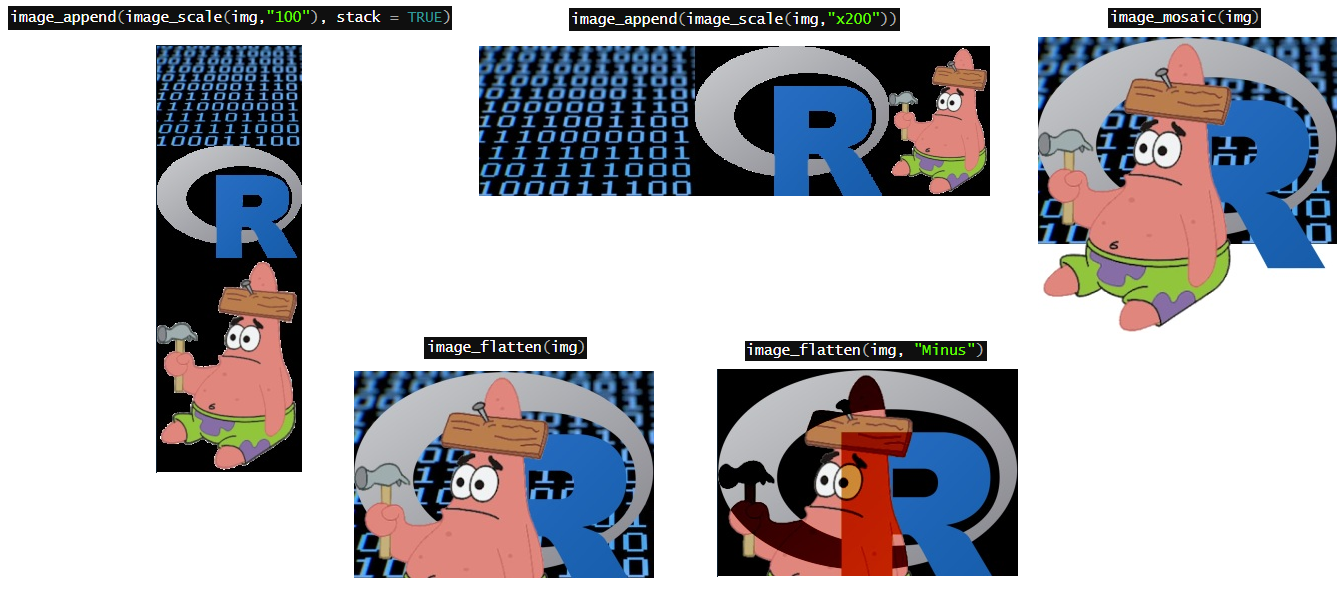
\includegraphics[width=4.4in]{IMAGENS/juntar_sobrepor}

\begin{center}
\tiny{Fonte: https://cran.r-project.org/web/packages/magick/vignettes/intro.html}
\end{center}

\end{frame}

\begin{frame}[fragile]{Imagens sobrepostas}
\protect\hypertarget{imagens-sobrepostas-2}{}

\begin{Shaded}
\begin{Highlighting}[]
\NormalTok{bigdatafrink <-}\StringTok{ }\KeywordTok{image_scale}\NormalTok{(}\KeywordTok{image_rotate}\NormalTok{(}
  \KeywordTok{image_background}\NormalTok{(frink, }\StringTok{"none"}\NormalTok{), }\DecValTok{300}\NormalTok{), }\StringTok{"x160"}\NormalTok{)}
\NormalTok{juntos <-}\KeywordTok{image_composite}\NormalTok{(}\KeywordTok{image_scale}\NormalTok{(}
\NormalTok{  bigdata, }\StringTok{"x330"}\NormalTok{), bigdatafrink, }\DataTypeTok{offset =} \StringTok{"+180+100"}\NormalTok{)}
\end{Highlighting}
\end{Shaded}

\end{frame}

\begin{frame}{Imagens sobrepostas}
\protect\hypertarget{imagens-sobrepostas-3}{}


\includegraphics[width=6.11in]{SLIDES_files/figure-beamer/5.4-1}

\end{frame}

\begin{frame}{Utilidade em gráficos}
\protect\hypertarget{utilidade-em-gruxe1ficos}{}

\small

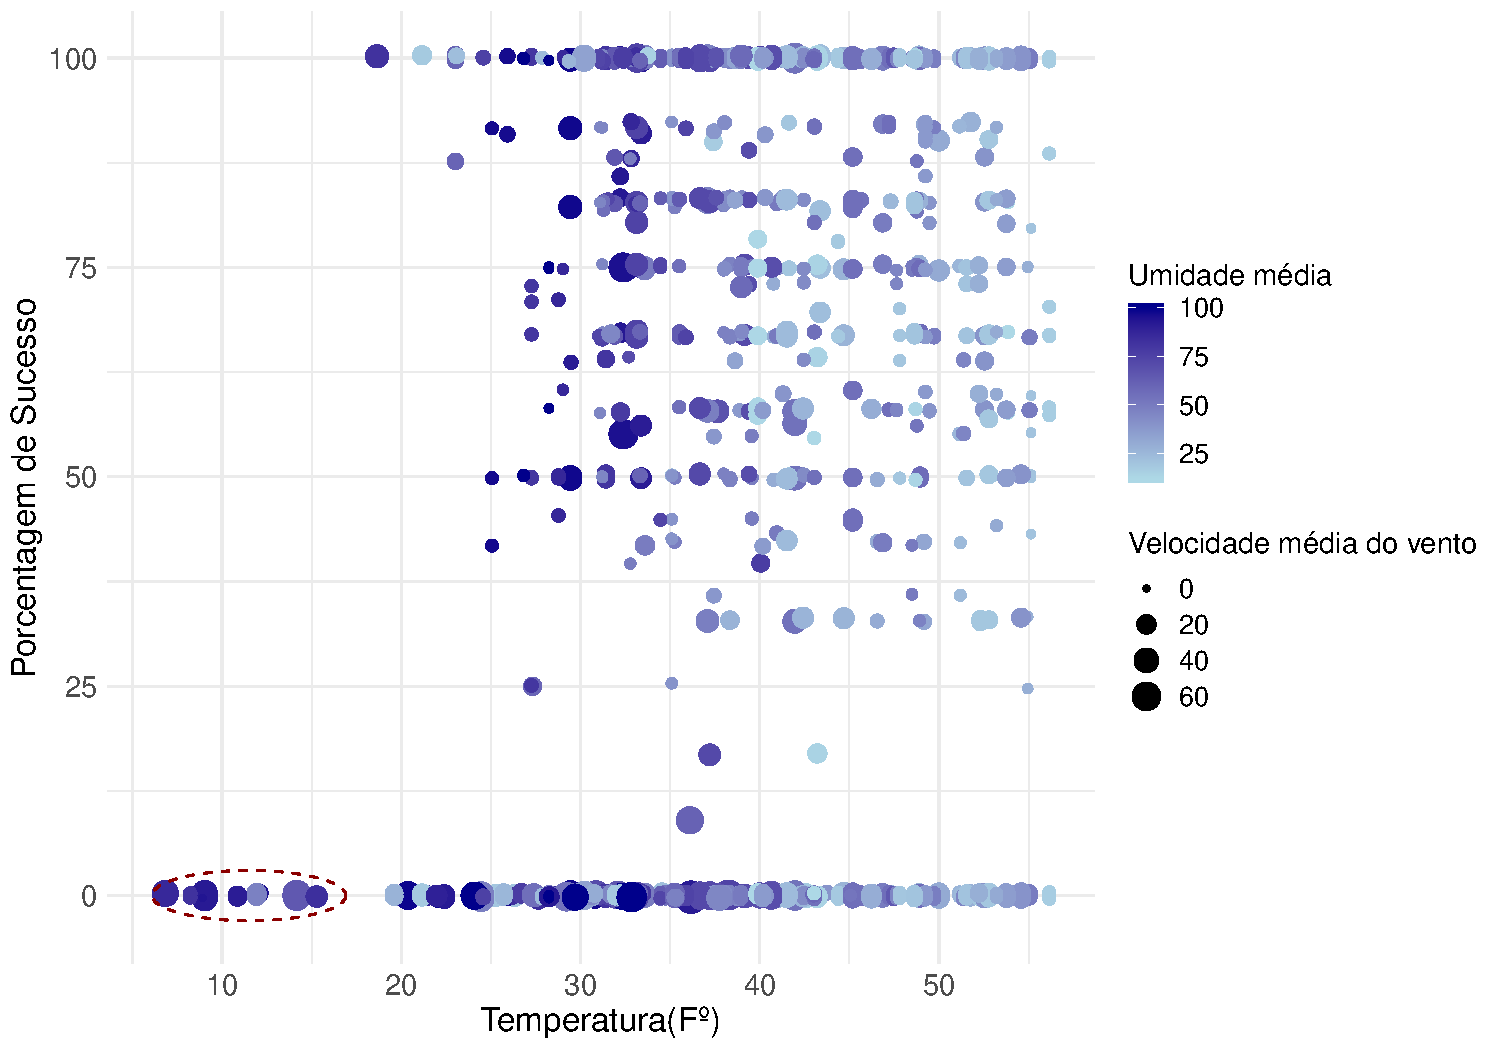
\includegraphics{SLIDES_files/figure-beamer/5.6-1.pdf}

\end{frame}

\begin{frame}[fragile]{Fraqueza na leitura de PDF}
\protect\hypertarget{fraqueza-na-leitura-de-pdf}{}

\begin{Shaded}
\begin{Highlighting}[]
\KeywordTok{require}\NormalTok{(pdftools)}
\NormalTok{temp <-}\StringTok{ }\KeywordTok{image_read_pdf}\NormalTok{(}\StringTok{"C:/Users/nick_/OneDrive/Área de Trabalho/image_analysis/Slide/IMAGENS/temp.pdf"}\NormalTok{)}
\NormalTok{temp <-}\StringTok{ }\KeywordTok{image_scale}\NormalTok{(temp, }\StringTok{"300x300"}\NormalTok{)}
\NormalTok{temp}
\end{Highlighting}
\end{Shaded}

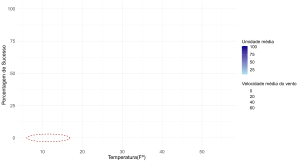
\includegraphics[width=4.17in]{SLIDES_files/figure-beamer/5.7-1}

\end{frame}

\begin{frame}[fragile]{Utilidade para sobreposição de imagens}
\protect\hypertarget{utilidade-para-sobreposiuxe7uxe3o-de-imagens}{}

\begin{Shaded}
\begin{Highlighting}[]
\NormalTok{graph <-}\StringTok{ }\KeywordTok{image_read}\NormalTok{(}\StringTok{"C:/Users/nick_/OneDrive/Área de Trabalho/image_analysis/Slide/IMAGENS/Rplot1.png"}\NormalTok{)}
\NormalTok{temp <-}\StringTok{ }\KeywordTok{image_read}\NormalTok{(}\StringTok{"C:/Users/nick_/OneDrive/Área de Trabalho/image_analysis/Slide/IMAGENS/low_temp.png"}\NormalTok{)}
\NormalTok{temp_graph <-}\StringTok{ }\KeywordTok{image_scale}\NormalTok{(}\KeywordTok{image_rotate}\NormalTok{(}\KeywordTok{image_background}\NormalTok{(}
\NormalTok{  temp, }\StringTok{"none"}\NormalTok{), }\DecValTok{340}\NormalTok{), }\StringTok{"x50"}\NormalTok{)}
\NormalTok{temp_graph}
\end{Highlighting}
\end{Shaded}


\includegraphics[width=0.69in]{SLIDES_files/figure-beamer/6-1}

\begin{Shaded}
\begin{Highlighting}[]
\NormalTok{juntos_}\DecValTok{2}\NormalTok{ <-}\KeywordTok{image_composite}\NormalTok{(}\KeywordTok{image_scale}\NormalTok{(}
\NormalTok{  graph, }\StringTok{"x600"}\NormalTok{), temp_graph, }\DataTypeTok{offset =} \StringTok{"+150+440"}\NormalTok{)}
\KeywordTok{image_write}\NormalTok{(juntos_}\DecValTok{2}\NormalTok{, }\DataTypeTok{path =} \StringTok{"juntos2.pdf"}\NormalTok{, }\DataTypeTok{format =} \StringTok{"pdf"}\NormalTok{)}
\end{Highlighting}
\end{Shaded}

\end{frame}

\begin{frame}{Utilidade para sobreposição de imagens}
\protect\hypertarget{utilidade-para-sobreposiuxe7uxe3o-de-imagens-1}{}

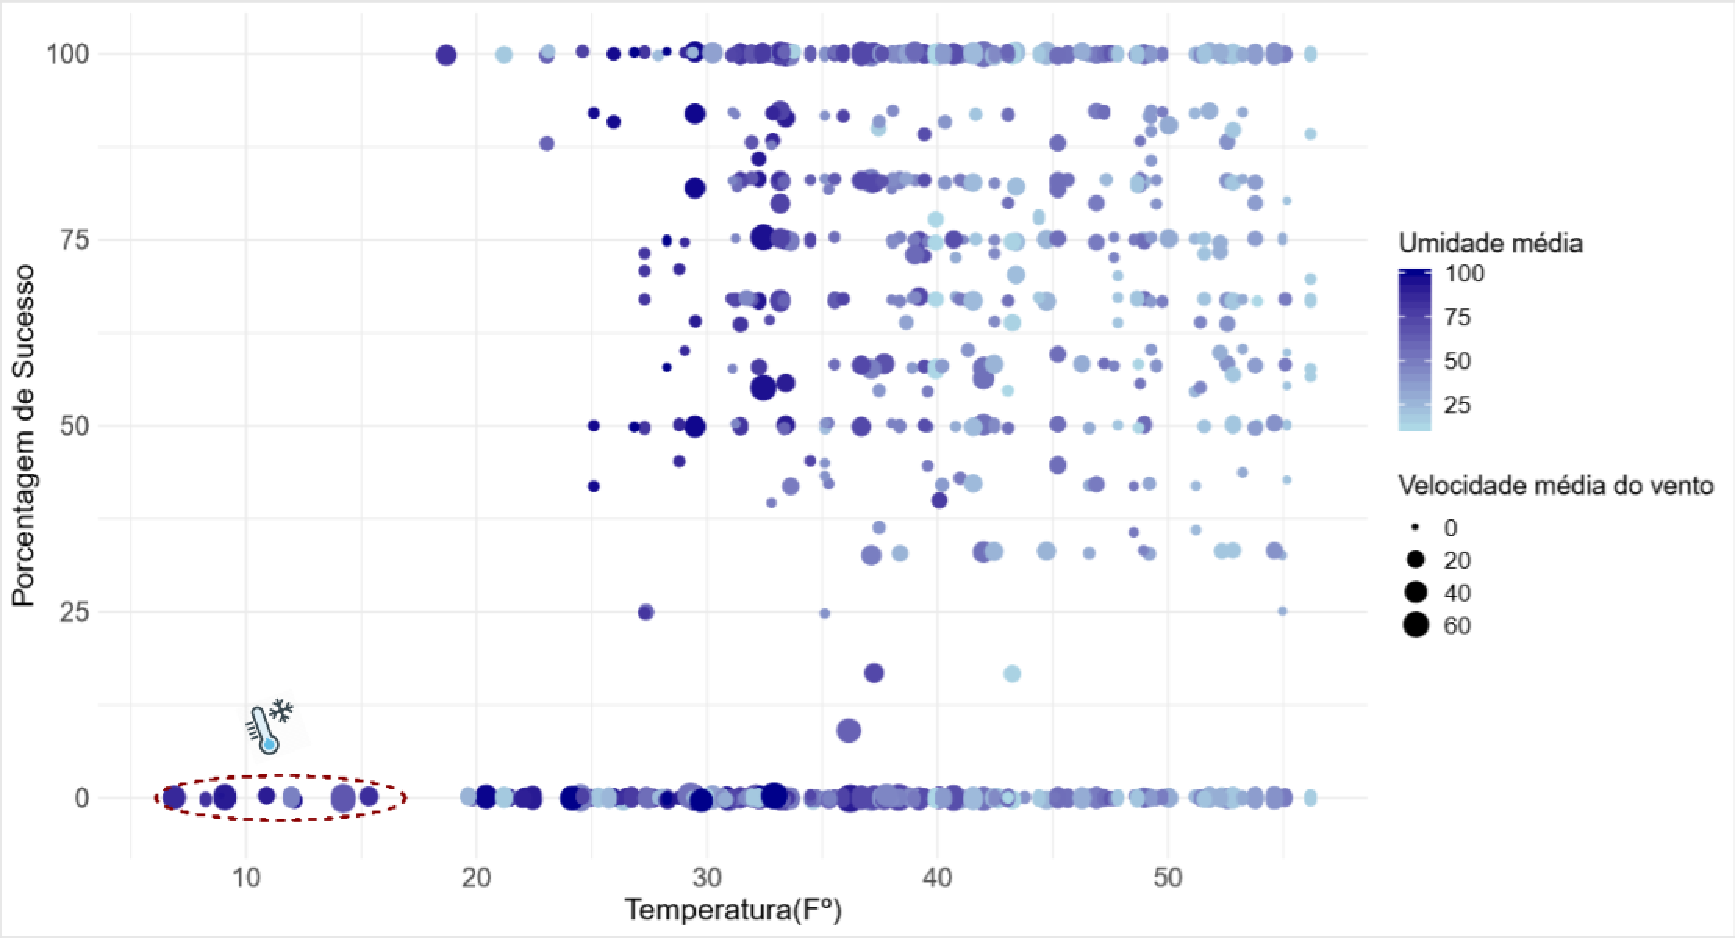
\includegraphics[width=4.4in]{juntos2}

\begin{center}
\tiny{Fonte: https://cran.r-project.org/web/packages/magick/vignettes/intro.html}
\end{center}

\end{frame}

\begin{frame}{Anotações em imagens}
\protect\hypertarget{anotauxe7uxf5es-em-imagens}{}

\end{frame}

\begin{frame}[fragile]{Gifs}
\protect\hypertarget{gifs}{}

\begin{Shaded}
\begin{Highlighting}[]
\NormalTok{earth <-}\StringTok{ }\KeywordTok{image_read}\NormalTok{(}\StringTok{"https://jeroen.github.io/images/earth.gif"}\NormalTok{) }\OperatorTok
\StringTok{  }\KeywordTok{image_scale}\NormalTok{(}\StringTok{"250x"}\NormalTok{) }\OperatorTok\StringTok{ }
\StringTok{  }\KeywordTok{image_quantize}\NormalTok{() }

\KeywordTok{length}\NormalTok{(earth) }
\end{Highlighting}
\end{Shaded}

\begin{verbatim}
## [1] 44
\end{verbatim}

\end{frame}

\begin{frame}[fragile]{Gifs}
\protect\hypertarget{gifs-1}{}

\begin{verbatim}
## # A tibble: 8 x 7
##   format width height colorspace matte filesize density
##   <chr>  <int>  <int> <chr>      <lgl>    <int> <chr>  
## 1 gif      200    155 sRGB       TRUE         0 72x72  
## 2 gif      200    155 sRGB       TRUE         0 72x72  
## 3 gif      200    155 sRGB       TRUE         0 72x72  
## 4 gif      200    155 sRGB       TRUE         0 72x72  
## 5 gif      200    155 sRGB       TRUE         0 72x72  
## 6 gif      200    155 sRGB       TRUE         0 72x72  
## 7 gif      200    155 sRGB       TRUE         0 72x72  
## 8 gif      200    155 sRGB       TRUE         0 72x72
\end{verbatim}

\includegraphics{SLIDES_files/figure-beamer/7.1-1.gif}

\end{frame}

\end{document}
